\section{Bridge the Gap between Language and Hardware Protections}
\label{sec:concept}

\subsection{The Challenges of Combining Language and Hardware Protections}

Language and hardware protections provide varying benefits
to application security:
Languages improve the internal security inside the applications,
while hardware provides the base defenses that cannot be easily overridden or bypassed.
Commonly security experts exploits both types of protections
to further harden the security of applications.
For example, hardware protections may take information from the language runtimes or compilers to enforce the security policies,
or language protections may rely on hardware protections to bootstrap the initial trust they need. 

However, the combination of language and hardware protections is more
like a trick of the trade for security experts:
the use of hardware protections is deeply buried in the design of language protections,
so that users (application developers) lose direct access
to the security guarantees and features provided by the hardware.
\fixme{Think of an example: Maybe TPM.}
The approaches of combining language and hardware protections are mostly ad-hoc to the use cases,
i.e., how one protection is used to improve or reinforce another.

There are two reasons for why combining language and hardware protections
is so inevitably hard.
First, hardware protections often have restrictions
on the languages that must be used
to access the security guarantees and features of the hardware.
For example, \sgx{} requires the loaded code to be implemented in C or C++,
or any languages that can compile applications into static binaries.
The restriction is not simply a design decision
made by the hardware or its SDK,
but a result of the fact that SGX requires a static image to guarantee the integrity of execution.
On the other hand, if the language used is a managed language like \java{},
accessing SGX hardware will be cumbersome,
because it is hard to provide any APIs to allow direct access to the SGX hardware,
to harvest its security guarantees
or to utilize its features.

\begin{figure}[t!]
\centering
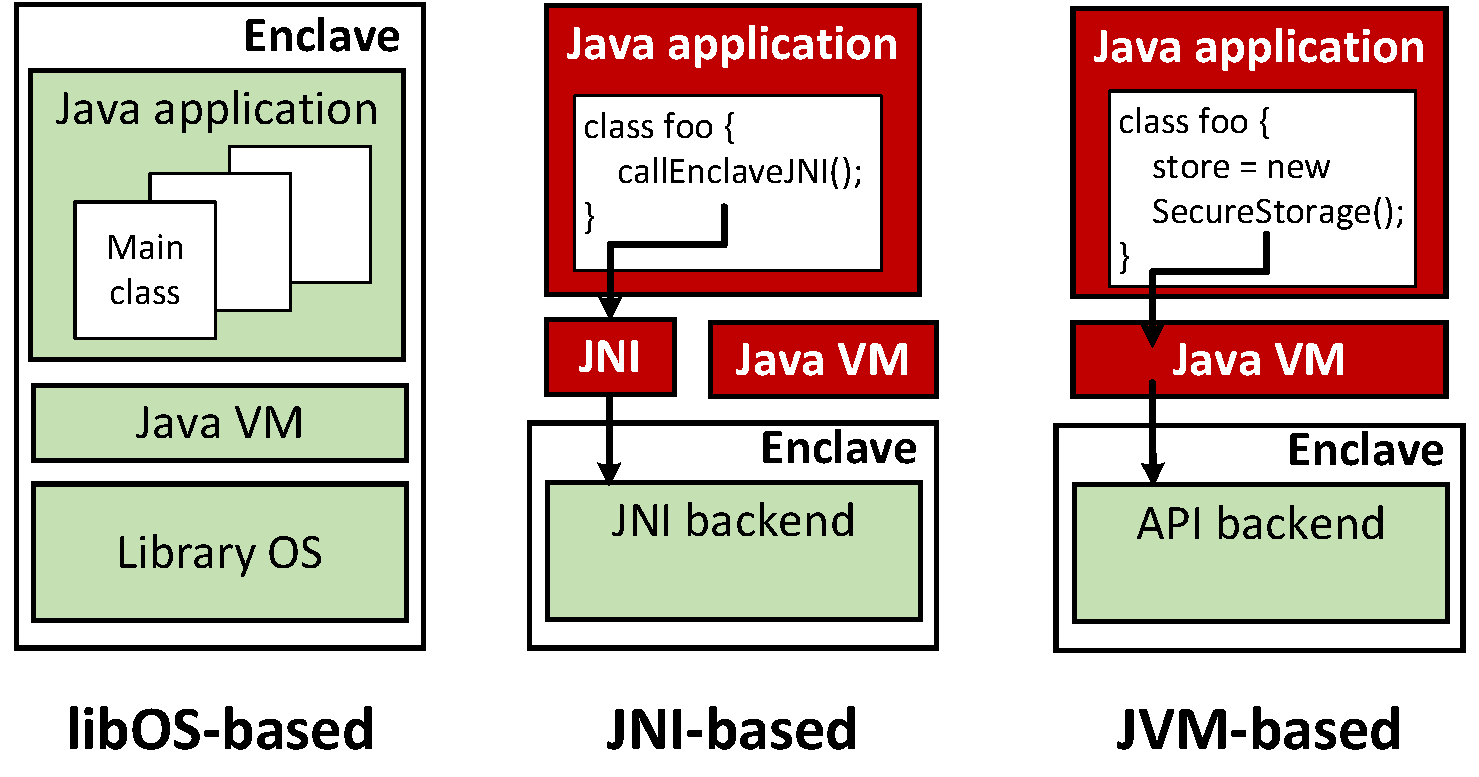
\includegraphics[width=\linewidth]{figures/alternatives.pdf}
\footnotesize
\caption{Alternative approaches to access \sgx{} hardware protection from \java{} applications.
The {\em libOS-based} approach runs the whole \java{} applications in the enclaves. 
The {\em JNI-based} approach uses JNI to run the security sensitive operations inside the enclaves.
The {\em JVM-based} approach requires the \java{} VM to provide APIs to support common use cases of the enclaves.
Green (light) boxes are trusted components and red (dark) boxes are untrusted.
}
\label{fig:alternatives}
\end{figure}


Figure~\ref{fig:alternatives} illustrates the alternative approaches
to access SGX hardware from \java{} applications:
The first approach is to run the whole \java{} applications with the \java{} VM inside the enclaves,
using a library OS ({\em libOS-based}).
This approach can secure applications as a whole,
but won't support any partitioned model for programming.
Another approach is to implement a JNI that create and interface with the enclaves
to run the security-sensitive operations ({\em JNI-based}).
The JNI-based approach is flexible enough for application developers
to implement the isolated components as well as the untrusted interface,
but requires developers to have the knowledge of
enclave implementation.
More importantly, the isolated components can only be developed in C or C++
language, so the applications lose the language protection of \java{} inside the enclaves.
A more plausible approach is to provide enclave-backed APIs
from the \java{} VM,
to support common use cases ({\em JVM-based})), such as a secure key-value store~\cite{vc3}.
Although the JVM-based approach can save the application developers' effort
of implementing isolated components,
the use cases is limited to the pre-defined operations provided by the \java{} VM or the companion frameworks.
Because the backend implementation (isolated components and untrusted interfaces) in the JVM-based approach is the same as the JNI-based approach,
the same language restriction also applies here. 

\subsection{Modeling Hardware Protections within Managed Languages}

To secure applications with the advantages from both \java{} language and \sgx{} hardware protection,
we must allow both isolated and untrusted components to be implemented in \java{}.
The two parts of the applications must be made to execute and interact
just as the currently supported model --- applications are implemented in C or C++ languages,
and compiled as static binaries.
Theoretically, if a use case of \sgx{} hardware is available for static binaries,
it can be established that the same use case
should be achievable within \java{} applications, with equal or stronger security guarantees.

As described earlier,
the \sgx{} hardware imposes language restrictions, which disallow \java{} applications to directly utilize enclaves
with a partitioned model,
where both isolated and untrusted components are \java{} classes.
However, the restrictions comes from the low-level {\em semantics} of
the \sgx{} hardware, which can be mitigated with system efforts.
The low-level semantics include the requirements for enclave creation,
the hardware instructions to interface with the enclaves,
and technical details of implementing secure applications to be loaded into the enclaves.

\begin{figure}[t!]
\centering
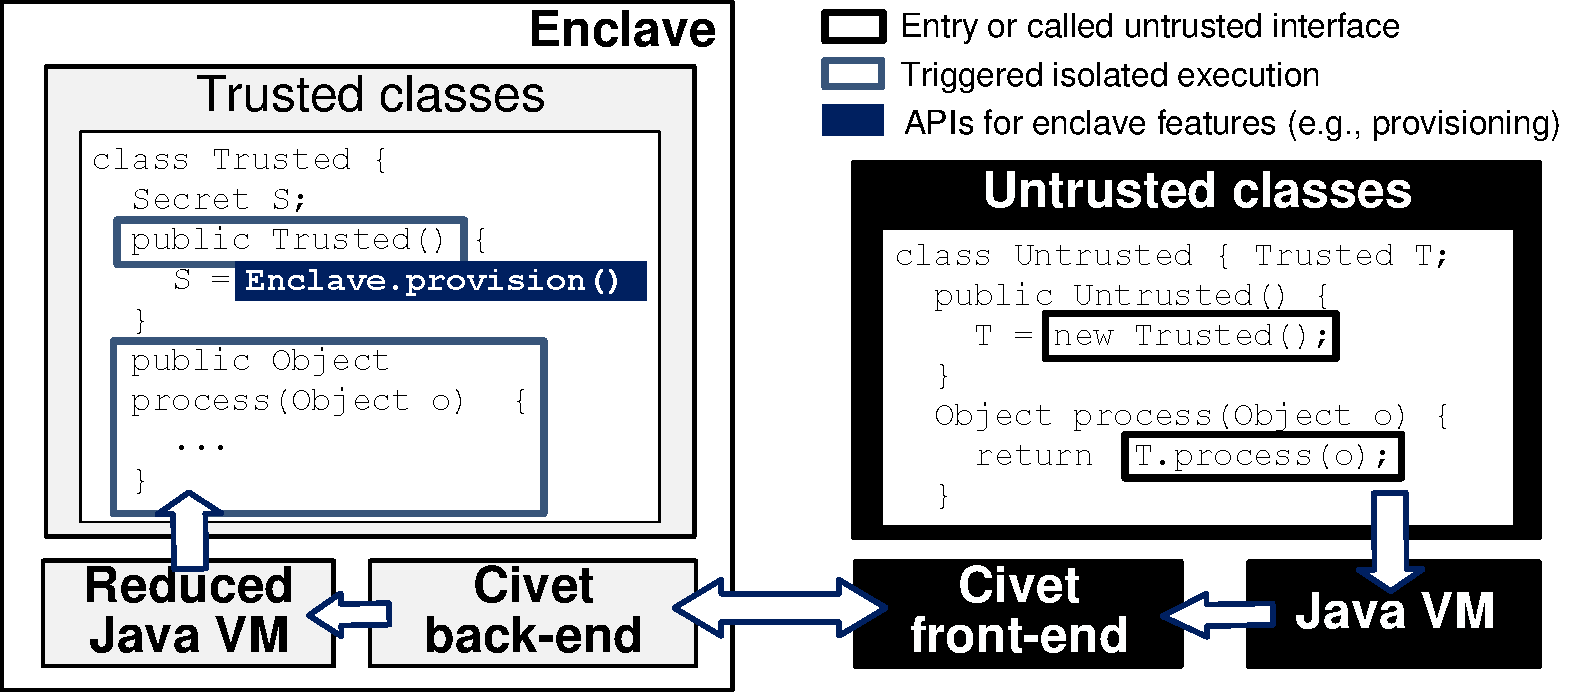
\includegraphics[width=0.9\linewidth]{figures/synthesis.pdf}
\footnotesize
\caption{How \sysname{} models the \sgx{} hardware protection for \java{} applications.
When an untrusted class ({\tt Untrusted}) calls the constructor of an isolated class ({\tt Isolated}),
\sysname{} creates the enclave and instantiates the isolated classes
inside the enclave. 
The public methods of the isolated class ({\tt process}) are exported
as the untrusted interface of the enclave, and the invocation of these methods will be re-routed into the enclave.
\sysname{} also provides APIs for accessing enclave features such as secure provisioning.
}
\label{fig:synthesis}
\end{figure}

\sysname{} transparently handles all the details of accessing \sgx{} hardware,
in behave of the loaded \java{} applications (as shown in figure~\ref{fig:synthesis}).
When \sysname{} is called to run isolated \java{} components,
it creates two worlds of \java{} execution --- one is in the enclave and the other is outside the enclave.
With the ability of running \java{} classes inside the enclave,
\sysname{} can support the partitioned model with both isolated and untrusted classes implemented as \java{} classes.

\begin{table*}[t!b!]
\centering
  \begin{tabular}{p{0.05in} >{\raggedright\arraybackslash}p{2.05in} >{\raggedright\arraybackslash}p{4.4in}}
  \toprule
  \multicolumn{2}{l}{\it Security guarantees or features} & {\it The modeling approach applied by \sysname{}} \\
  \midrule
  \midrule
  \multicolumn{3}{l}{\bf Natively provided by the \sgx{} hardware (including the SDK):} \\
  \midrule
  & Isolating security-sensitive components &
  Asking developers to identify multi-level sensitivity, by marking the {\em entry classes}. Complete separation between isolated and untrusted classes.
  \\
  \midrule
  & Secure entry / exit of enclaves &
  Exporting public methods of isolated classes. Arguments are type-checked.
  \\
  \midrule
  & Integrity of the execution environment & 
  Packaging all supporting classes into a signed JAR.
  \\
  \midrule
  & Attestation \& secure provisioning & 
  Providing class {\tt Enclave}, to create secure channels and exchange attestation.
  \\
  \midrule
  \midrule
  \multicolumn{3}{l}{\bf Improvement from combining of \java{} language and the \sgx{} hardware protection:} \\
  \midrule
  & Memory safety \& control flow integrity &
  Naturally provided by \java{} language.
  \\
  \midrule
  & Reducing the enclave TCB &
  Automated partitioning based on class dependencies.
  \\
  \midrule
  & Preventing information flow leakage &
  Tracking information flow in trusted classes, only allow releasing the information if not tainted or declassified by developers.
  \\
  \midrule
  & Code confidentiality & Dynamically loading provisioned classes.
  \\
  \end{tabular}
  
\footnotesize
\caption{
The approaches applied by \sysname{} to model the security guarantees and features of the \sgx{} hardware, and to enhance the security by combining language and hardware protections.
}
\label{tab:features}
\end{table*}


Even though \sysname{} hides the low-level semantics of the \sgx{} hardware from the applications,
the applications still have full access to the security guarantees ({\em what is secured?}) and features ({\em how is it secured?}) provided by the the \sgx{} hardware.
We do so by identifying the high-level goals of these guarantees and features,
and remodel the goals in the \java{} language.
The underlying mechanisms of these goals is the original guarantees and features provided by the \sgx{} hardware.

We discuss each security guarantee or features of the \sgx{} hardware,
and how they are actually modeled in \sysname{} as follows.

\paragraph{Isolated execution of security-sensitive components}
The \sgx{} hardware ensures components with higher security sensitivity
to be executed inside the enclave
and completely isolated from the components that are less security sensitive.
The isolated components shall not share any data with the untrusted components unless the isolated components decide
to flow the data out of the enclave.  

\sysname{} models this guarantee by asking the developers to make
the classes that they believe to be security sensitive.
Note that only the top-most classes that interact with the untrusted components have to be identified --- we can these classes as the {\em entry classes}.
After developers identifying the multi-level security sensitive with an application, \sysname{} uses a building tool to partition the application
based on the developers' hint.
The partition completely separates the \java{} classes for the isolated components from the classes for the untrusted components.
The execution of these isolated classes will be fully jailed inside the enclave, and any invocation of the methods exported by the isolated classes
from the untrusted classes
will be re-routed into the enclave.
The returned values of the invoked methods will be routed back to
the untrusted classes,
either as proxies of the actually returned instances (if the instances are not yet safe to release from the enclave) or the actual values.

\paragraph{Secure entry and exit of the enclave}
The \sgx{} hardware ensures that the enclave only has fixed number of entry points (exactly one location where the execution starts, but multiple pre-defined locations that the execution can jump to). 
The untrusted components must be forbidden to jump to random code in the enclave.
Moreover, if the isolated component want to exit the enclave,
it must explicit call the exit instruction ({\tt EEXIT}) to make sure
the control flow won't be manipulated to leave the enclave.

\sysname{} models this guarantees by exporting all the public methods of the isolated classes
(including constructors, static and non-static methods) as the entry points or untrusted interfaces.
When the untrusted component calls a constructor or static method of an isolated class,
the execution inside the enclave is triggered,
either to instantiate the class or perform other operations.
If a proxy of an isolated instance is returned to the untrusted components,
the untrusted components can keep it or pass it around.
As soon as any untrusted components call one of the public methods on the proxy, the execution re-enter the enclave and start the isolated execution.

Exporting public methods as the entry points or the untrusted interface
is assumed to be reasonably secure in \sysname{}.
First, only for the entry classes (the top-most classes of the enclave),
the constructors or static method will be exported.
Because developers have expressed that these classes are the ones that interact with the untrusted classes, it is safe to allow the untrusted components to calls these methods and trigger execution in the enclave.
Second, even if the public non-static methods can be called
upon isolated classes, the untrusted components can only call upon the proxies,
which are essentially returned values from the previous method calls.
Without the proxy, the untrusted components can never call the public methods
on random instances in the enclave, if the instances are never returned to the untrusted components.

\paragraph{Integrity of the execution environment}
The \sgx{} hardware must guarantee the execution of the isolated components
is exactly the same as developed, tested and verified by the application developers.
The \sgx{} hardware verify the cryptographic measurement of loaded binaries
at the creation of the enclave,
and can generate attestation that the enclave is created with such measurement.
The purpose of the guarantee is to prevent code injection,
unless the isolated applications are tricked into loading the code by the attackers.

\sysname{} models this guarantee by creating a snapshot of developers'
execution environment, including the version of \java{} VM,
checksums of any infrastructure binaries,
and the minimal supporting classes for the isolated component. 
\sysname{} packs all these files into a JAR file and sign it with the developers' private key.
When \sysname{} creates an enclave, the hardware measurement of the enclave includes only the infrastructure, as the \java{} VM and the \sysname{} back-end.
Once the enclave is created, the \sysname{} back-end must  
check whether the JAR file loaded has the correct signature.

\paragraph{Secure provisioning and attestation}
The \sgx{} hardware provides the isolated components the feature to generate attestation to prove the integrity of its execution,
and to use the attestation to securely exchange
security sensitive information such as encryption keys from the remote trusted host.

\sysname{} models these features by providing a class called {\tt Enclave}, with the APIs that service attestation and provisioning requests.
The {\tt Enclave} APIs are wrapper to the low-level semantics required by the \sgx{} hardware,such as exchanging the attestations with remote hosts and verifying them, or 
securing the channels after attesting the other side of communication.
Because the works are completely hidden beneath the APIs,
the developers are spared from all the cryptographic details during the process of attestation and provisioning.

\vspace{0.15in}
Table~\ref{tab:features} lists the security guarantees and features of
the \sgx{} hardware
that are modeled by \sysname{} for \java{} applications.
The table also lists other guarantees and features
that are not natively provided by the \sgx{} hardware
but enhanced by \sysname{} after combining the language and hardware protection, which will be discussed in the later sections.  

\subsection{Hardening Hardware Protections with Language Protections}

\sysname{} models the high-level security guarantees and features
of the \sgx{} hardware in the \java{} language,
allowing the developers to directly utilize these guarantees and features
while still implementing applications in \java{}.
By bridging the gap between language and hardware protections,
\sysname{} creates opportunities to combine \sgx{} hardware protections
and security benefits given by \java{} as a managed language.

Several security enhancements come naturally with running \java{} classes
in the enclave. \java{} applications are known to be immune to memory corruption bugs such as buffer or heap overflow.
With any type casting in the \java{} applications, \java{} perform strict type-checking on the objects to be casted.
Type-checking prevents corruption of object either in the isolated components,
or when receiving arguments from the untrusted interfaces.
Memory corruption bugs are constant threats to applications
implemented in C or C++ languages,
but \java{} applications naturally defend against these vulnerabilities.

Similar as the memory corruption bugs,
\java{} classes are also immune to control flow attacks.
applications implemented in C or C++ languages inevitably face the risk of ROP (return-oriented programming) attacks,
where attackers can manipulate the control flow by corrupting the applications' stacks or heaps.
Since \java{} classes can defend against memory corruption,
attacks cannot manipulate the control flow by overriding the return pointers or function pointers.

Note that although memory corruption bugs and control flows attacks are forbidden in \java{} classes,
these vulnerabilities can still exist in the \java{} VM and JNI.
In \sysname{} we assume \java{} VM and JNI must be fully trusted,
and we leave it as a future work to secure these components.

For isolated components in the enclaves, memory corruption bugs and control flow attacks are just as dangerous as for other applications.
Because the isolated components are fully trusted by the CPU,
they can access any memory that are set to proper permissions, including the memory outside the enclaves.
Even if a vulnerable component is exploited to copy all the enclave secret out of the enclaves, no hardware solution can effectively stop the exploitation.
Even though isolated components cannot directly jump out of the enclave,
control flow attack can still manipulate the components to jump to certain locations internally and perform malicious operations. 
Therefore, preventing memory corruption bugs and control flow attacks
can be a strong reason for application developers
to choose \java{} language instead of C/C++ to implement the isolated components.

\paragraph{Reducing the enclave TCB}
A \java{} applications often yield a huge TCB, including the \java{} VM,
JNI and supporting classes that come in bulk.
For example, a \java{} applications executed by \jvmname{}
will load the \java{} VM binaries up to 40MB \fixmets{find out actual numbers}. The classes in the standard \java{} VM libraries such as {\tt rt.jar} includes more than 18,000 classes, and the size of the package is more than 30MB.
On the other hand, the actual classes needed by an application from {\tt rt.jar}
can be as less as 1,000 classes.
Majority of the classes provided from {\tt rt.jar},
--- even though they may never be loaded into the enclave ---
still remains in the TCB.

Having unnecessary binaries and classes in the TCB of the enclave
can aggravate the risk of being attacks.
First of all, the huge amount of code loaded into the enclave
increase the opportunity of having gadgets that can be exploited in ROP attacks,  
which can still happen in the \java{} VM or JNI.
Even though most of the \java{} classes have static footprint of their supporting classes,
many of them still dynamically load classes, such as directly calling the class loader, or specifying providers to the \java{} cryptography framework.
Having huge TCB as \java{} classes in the enclave still intensify
the risk of attacks, even though \java{} classes are immune to control flow attacks. 

\sysname{} largely reduce the supporting classes that can be loaded into the enclave,
by partitioning out the necessary classes from all the libraries in the developers' class paths, into the enclave image.
When the enclave is created, the \java{} VM will not load any existing libraries such as {\tt rt.jar} from the host system,
but instead only search classes in the signed enclave image.
Minimizing the supporting classes that can be loaded into the enclave
guarantees that all the classes that are included in the TCB
are actually required by the isolated components,
and come from a trusted source such as the developers' execution environment. 

Note that we do not partition the JNI within the \java{} VM binaries.
We assume partitioning out the JNI functions that are required by the isolated classes
is fully feasible with some manageable efforts.
Moreover, the \java{} classes can be potentially partitioned at a smaller granularity than the whole classes, such as the methods and fields, which can even further reduce the TCB.
We leave these potential improvements as future works. 

\paragraph{Enforcing information flow control in enclaves}


\paragraph{Providing code confidentiality}
